\documentclass[../main.tex]{subfiles}

\begin{document}
Dentro del mundo del Machine Learning existen numerosas herramientas de trabajo, siendo un entorno que se renueva a una velocidad de vértigo. \newline

El "verano" que atraviesa la Inteligencia Artificial en general y la Visión Artificial en particular provocan que numerosas instituciones, empresas y particulares apuesten por desarrollar nuevas herramientas o mejorar las ya existentes. Algunos de esos contribuyentes son actores de la industria tan destacados como Google, Facebook y NVIDIA.
\newline

Por otra parte, en este Trabajo Final de Grado se han utilizado herramientas principalmente de código abierto y con amplia documentación, las cuales se detallan a continuación.
\section{Python}
Python es un lenguaje de programación que apareció en 1991, diseñado por Guido Van Rossum. Actualmente administrado por la Python Software Foundation y distribuido mediante una licencia de código abierto denominada Python Software Foundation License. \newline

En los últimos años ha ganado mucho peso en todos los ámbitos de la Informática, debido a su filosofía centrada en la legibilidad del código y su facilidad de aprendizaje. Sus características principales son las siguientes:
\begin{itemize}
  \item Soporta programación estructurada, orientada a objetos, imperativa y funcional, sin forzar al usuario a decantarse por ninguno de ellos y pudiendo cambiar entre ellos en cualquier momento. Este enfoque aúna las ventajas de cada paradigma, facilitando a los programadores utilizar la solución que deseen sin verse limitados por el lenguaje de programación.
  \item Posee un diseño que facilita la extensión del mismo y la interoperabilidad con otros lenguajes de programación, estimulando la creación de librerías y módulos compatibles con Python.
  \item A diferencia de otros lenguajes, su código es interpretado por un intérprete. Este enfoque proporciona un mayor soporte a la multiplaforma, existiendo implementaciones de Python escritas en lenguajes como C, Java o C\# para una gran cantidad de sistemas operativos.
  \item Proporciona un modo interactivo similar a una terminal de comandos, lo que permite un desarollo más cómodo para el programador al probar bloques de código independientemente de forma sencilla.
  \item Su sistema de tipos es fuertemente tipado y dinámico, lo que aporta una mayor seguridad en las operaciones del programa sin renunciar a facilitar el desarrollo y el mantenimiento del mismo.
  \item Incorpora soporte para la instalación de módulos mediante la herramienta pip, utilizada en este Trabajo Final de Grado para facilitar la instalación de las dependencias del sistema implementado.
\end{itemize}

\section{TensorFlow}
TensorFlow es una librería de cálculo numérico orientada a la computación distribuida, creada por Google y bajo el amparo de la licencia de código abierto Apache 2.0 desde noviembre de 2015.\newline 

Ha ganado mucho protagonismo en los últimos años ya que principalmente facilita el uso de tarjetas gráficas para acelerar la computación que necesitan los modelos de Machine Learning. Sus principales características son:
\begin{itemize}
    \item Permite variar el hardware de forma trasparente al programador, sin tener que realizar código adicional o transformarlo para las diferentes implementaciones. En otras palabras, implementa el Principio de inversión de dependencias, logrando que el programador dependa únicamente de abstracciones y no de los detalles de implementación.
    \item Internamente utiliza grafos de flujo de datos, lo que permite ciertas optimizaciones y un procesado vectorial de los propios datos, aumentando la eficiencia del software. Con la publicación de TensorFlow 2.0 el 30 de septiembre de 2019, no es necesario programar forzosamente mediante dichos grafos, permitiendo el uso de un paradigma imperativo (\textit{Eager Execution}) más intuitivo de cara al programador.
    \item Proporciona API para los siguientes lenguajes: Python (utilizada en este Trabajo Final de Grado), C++, Haskell, Java, Go y Rust.
\end{itemize}

\section{Tensorboard}
Tensorboard es la interfaz gráfica incluida con TensorFlow para facilitar la comprensión del software implementado. Posee herramientas para la visualización de gráficas asociadas a las métricas del modelo, lo que permite evaluar de forma rápida el proceso de aprendizaje del modelo ya que indica, además de la métrica, los metadatos que queramos además del tiempo transcurrido de ejecución. \newline

\begin{figure}[h!]
    \centering
    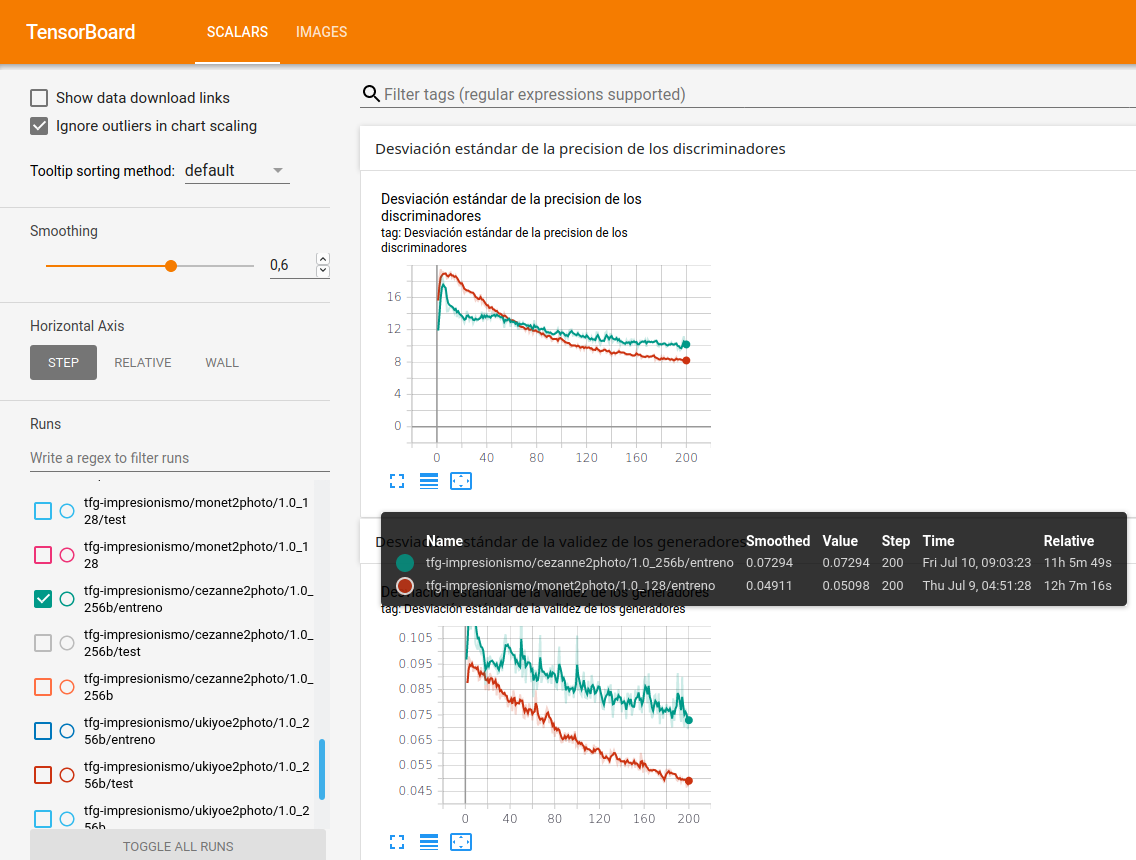
\includegraphics[width=0.75\textwidth]{imagenes/Tensorboard_graficas.png}
    \caption{Ejemplo de las gráficas proporcionadas por Tensorboard}
    \label{fig:tensorboard_descripcion_graficas}
\end{figure}

Asimismo dispone de opciones para visualizar imágenes relacionadas con el modelo, el grafo de computación ejecutado por TensorFlow, histogramas y distribuciones.

\begin{figure}[h!]
    \centering
    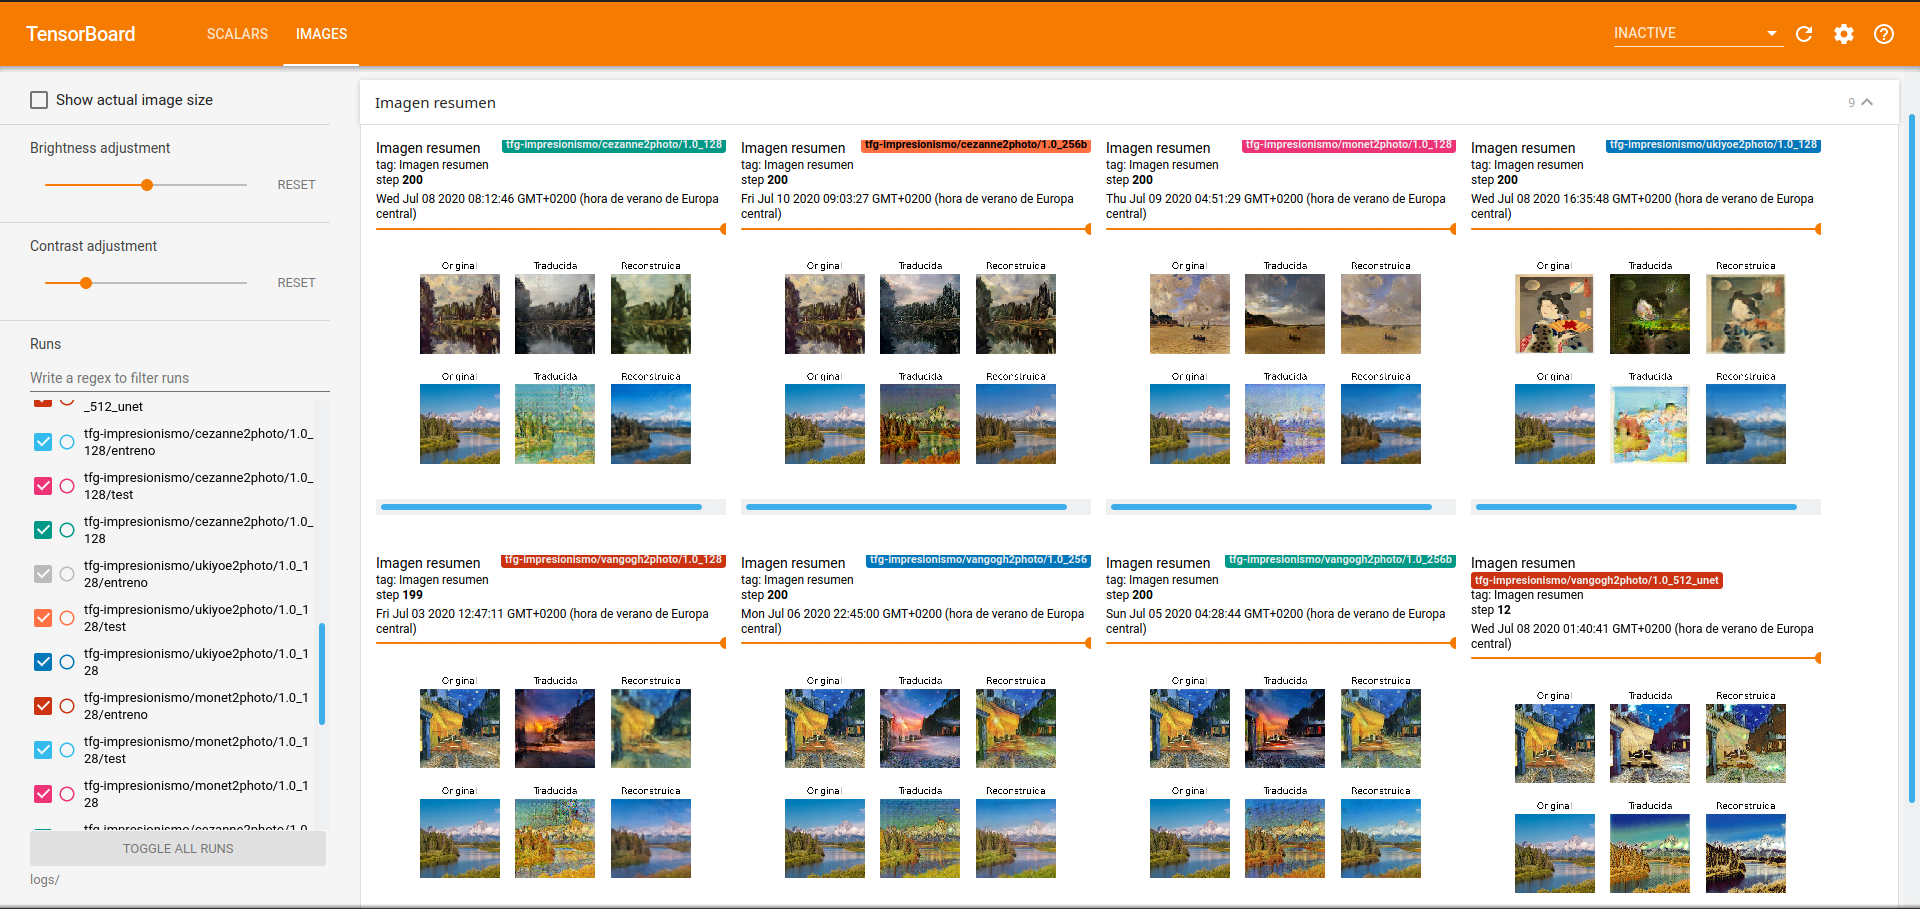
\includegraphics[width=1\textwidth]{imagenes/Tensorboard_imagen_resumen.png}
    \caption{Ejemplo de la visualización de fotos mediante Tensorboard}
    \label{fig:tensorboard_descripcion_imagenes}
\end{figure}

\section{Keras}
Keras es una API de Redes Neuronales que permite un desarrollo y mantenimiento cómodo y sencillo de las mismas. Desarrollada por François Chollet, fue lanzada el 27 de marzo de 2015 bajo la licencia de código abierto MIT. Dicha interfaz puede funcionar bajo TensorFlow, Theano y Microsoft Cognitive Toolkit, abstrayendo el modelo del \textit{background} computacional.
\newline

La combinación de TensorFlow con Keras es ampliamente utilizada en el sector debido a su sencillez de uso, potencia y eficacia. De hecho, TensorFlow en su versión 2 renunció a sus API de modelos predefinidos para ofrecer una integración completa y óptima con Keras.

\section{CUDA}

CUDA son las siglas de \textit{Compute Unified Device Architecture} (Arquitectura Unificada de Dispositivos de Cómputo), una plataforma para realizar procesamiento paralelo mediante las GPU de NVIDIA, creada en el año 2007. Esta herramienta permite utilizar las ventajas del paralelismo masivo que ofrecen las GPU mediante un dialecto de C, si bien existen enlaces para poder usarla desde Python, Fortran y MATLAB.
\newline

Con esta tecnología, podemos paralelizar de forma sencilla nuestras aplicaciones. Así mismo dispone de una extensión, llamada cuDNN, que optimiza las aplicaciones de Redes Neuronales, reduciendo aún más los tiempos de cómputo. De hecho, en este Trabajo Final de Grado es utilizada indirectamente, ya que es la plataforma que usa TensorFlow para paralelizar sus operaciones; si bien requiere una configuración un tanto problemática. Dicha situación se detallará en la sección \ref{sec:dependencias}

\section{Google Cloud Plataform}

Google Cloud Plataform es la plataforma de computación en la nube propiedad de Google, en la que se ofertan todo tipo de servicios. Mediante esta herramienta, los usuarios pueden contratar servicios de forma rápida y flexible, sujetos únicamente al pago por uso de los mismos. Entre otros, provee servicios de Inteligencia Artificial, Big Data y almacenamiento, además de máquinas virtuales totalmente configurables y de elevado rendimiento. \newline

\begin{figure}[h!]
    \centering
    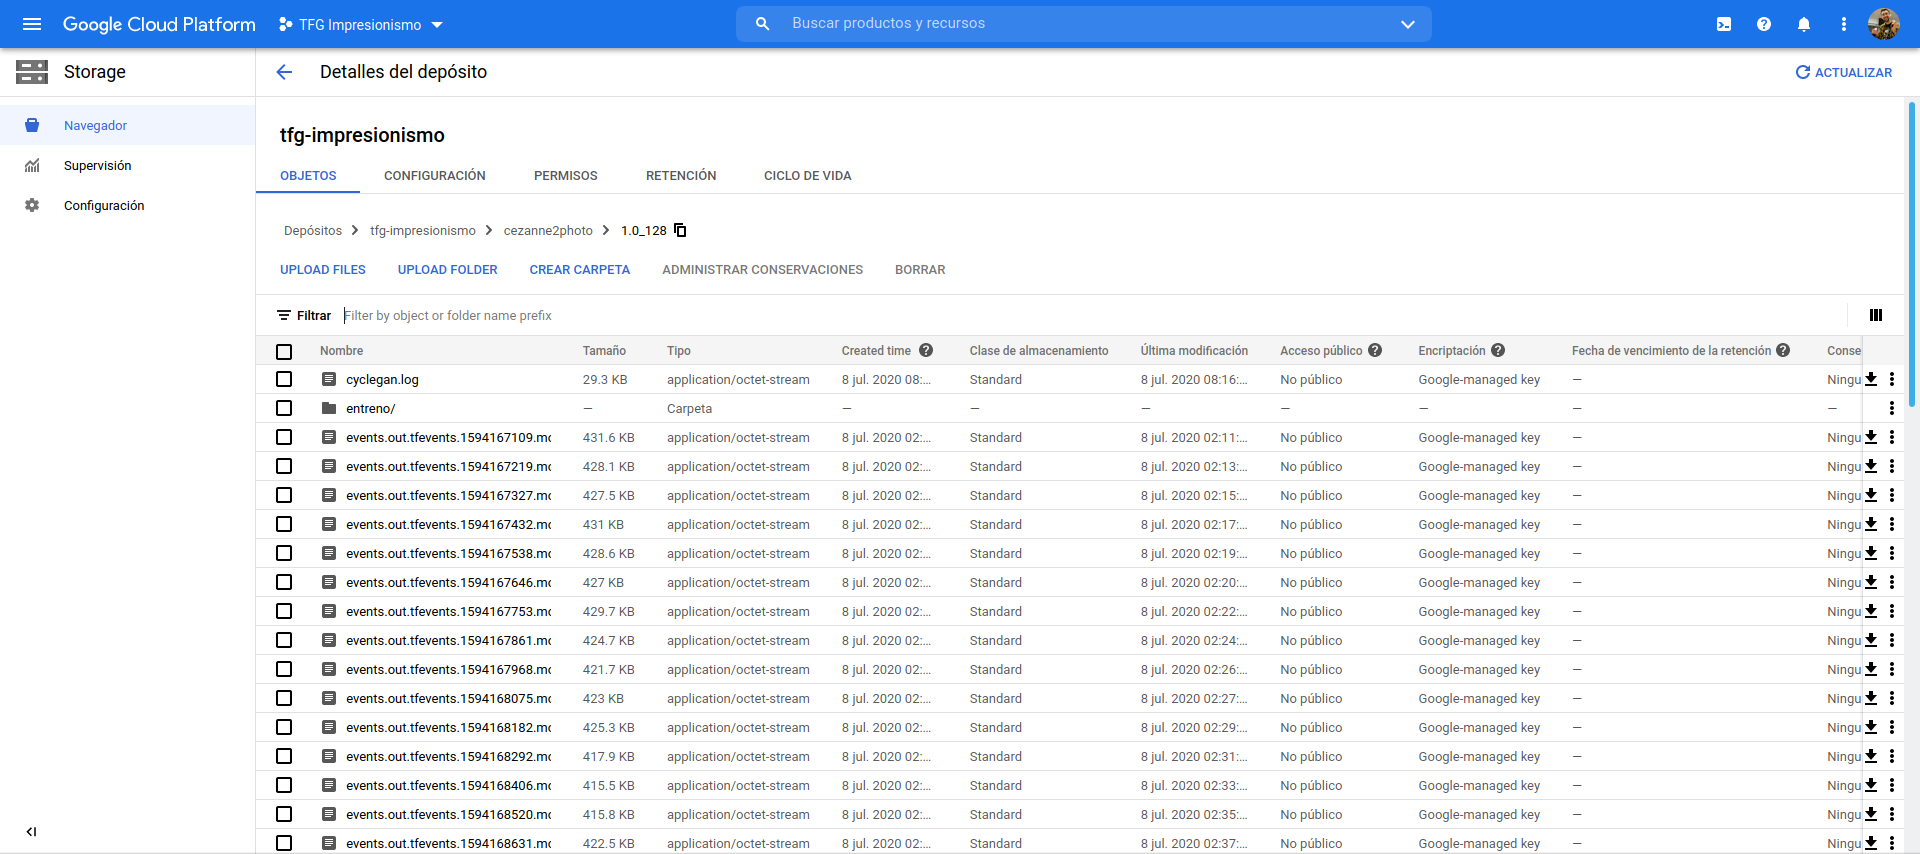
\includegraphics[width=1\textwidth]{imagenes/gcp_logs.png}
    \caption{Ejemplo de visualización de una instancia del servicio de almacenamiento de Google Cloud Plataform}
    \label{fig:gcp_logs}
\end{figure}

En este Trabajo Final de Grado se ha utilizado esta plataforma para acceder a las GPU y TPU de Google, las cuales permiten acelerar en gran medida los tiempos de entrenamiento del sistema propuesto.

\begin{figure}[h!]
    \centering
    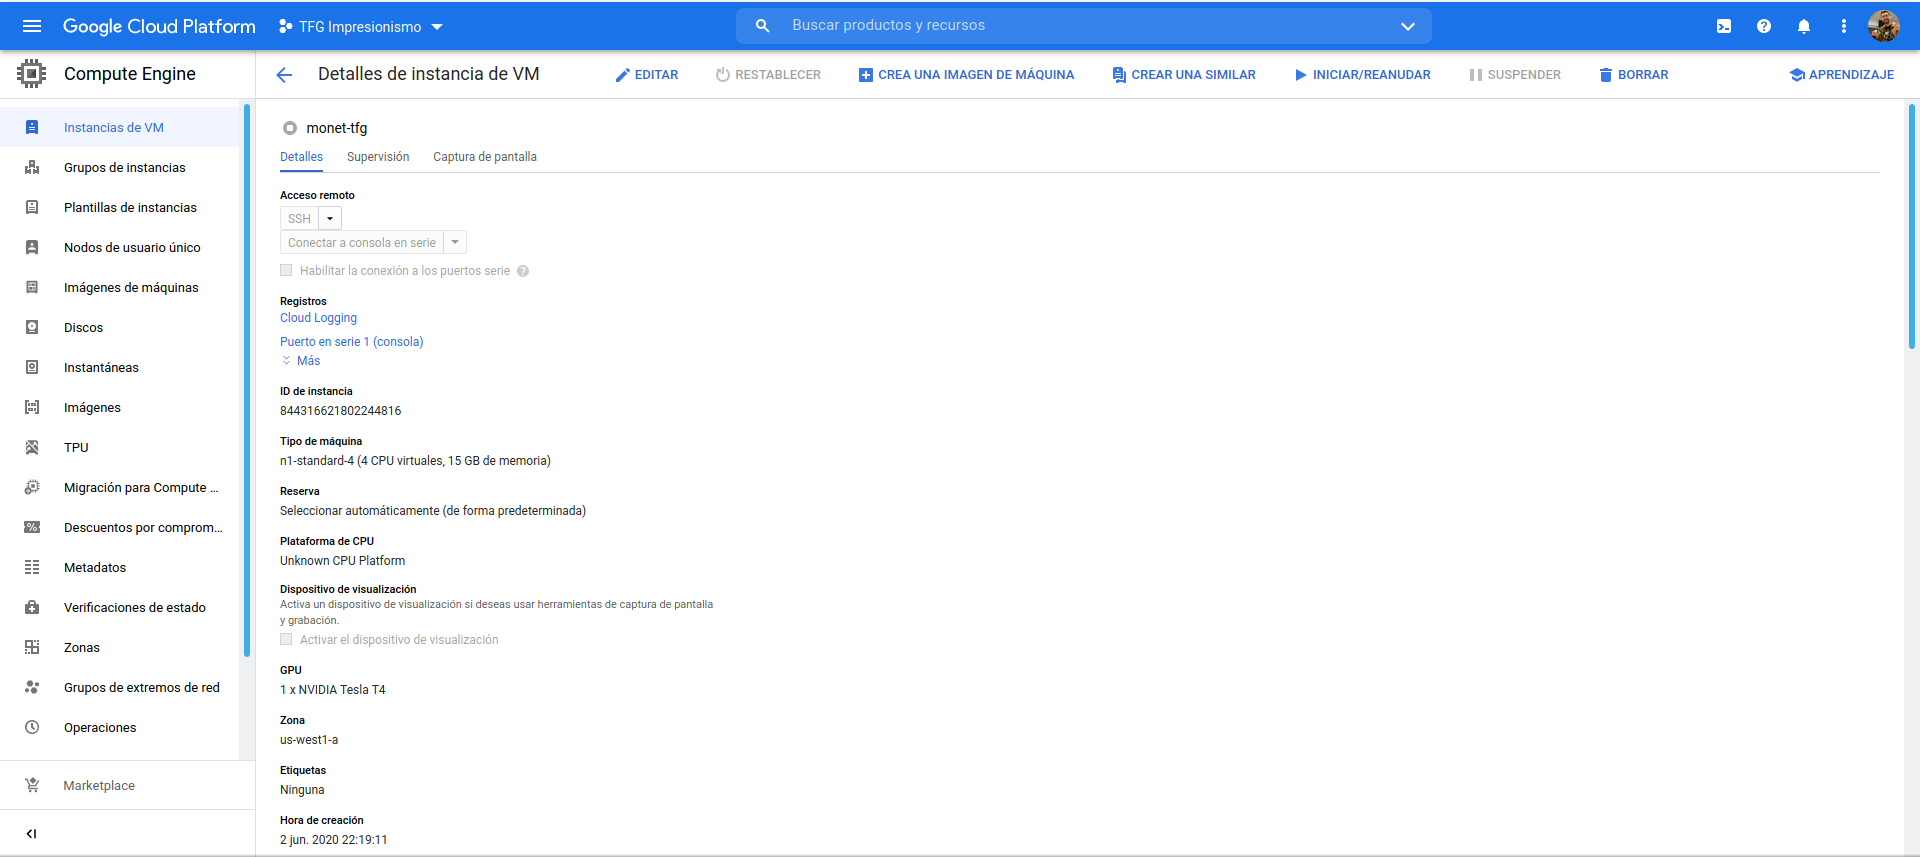
\includegraphics[width=1\textwidth]{imagenes/gcp_mv.png}
    \caption{Visualización de la descripción de la máquina virtual utilizada en este TFG alojada en Google Cloud Plataform}
    \label{fig:gcp_mv}
\end{figure}

\section{Flask}
Flask es un \textit{microframework} elaborado para desarrollo web mediante Python, creado por Armin Ronacher y liberado bajo la licencia de código abierto BSD. A diferencia de otros frameworks, Flask está pensado para crear aplicaciones web rápidamente, con una curva de aprendizaje suave para el programador; lo que permite desarrollar servicios de forma ágil y rápida.
\newline

Además añade soporte para la creación de API REST de forma extremadamente sencilla, que es el uso que le daremos en este Trabajo Final de Grado.

\section{Git y GitHub}

Git es un sistema de control de versiones \textit{open source} diseñado por Linus Torvalds (conocido por ser el artífice de Linux). Este sistema de control de versiones se caracteriza por su concepción distribuida, lo que permite prescindir de un servidor si así lo deseamos. Diseñado para el desarrollo no lineal de proyectos, fue desarrollado para la gestión del núcleo de Linux, lo que junto a su velocidad, eficiencia y facilidad de uso lo ha converido en uno de los sistemas más utilizados en todo el mundo.

Por otra parte, GitHub es una plataforma propietaria diseñada principalmente para el alojamiento remoto de repositorios Git. Si bien no es necesaria para utilizar Git, ha adoptado una inmensa popularidad debido a que nos permite tener repositorios privados (ahorrando a los desarrolladores el despliegue y mantenimiento de un servidor) sin renunciar a crear repositorios públicos con los que compartir nuestro código hacia la comunidad. En este \tfg se ha utilizado tanto Git como GitHub para el control de versiones de la implementación \textit{software}.

\end{document}
